\subsection{Syntactic Sugar}
\begin{frame}[fragile]
\begin{lstlisting}[frame=htrbl]
(|>>>|) :: (Arrow arr) => [arr a b] -> [arr b c] -> [arr a c]
(|>>>|) = zipWith (>>>)
\end{lstlisting}

\begin{lstlisting}[frame=htrbl]
(|***|) :: (Arrow arr, ...) =>
	arr a b -> arr c d -> arr (a, c) (b, d)
(|***|) = parEval2 ()
\end{lstlisting}

\begin{lstlisting}[frame=htrbl]
(|&&&|) :: (Arrow arr, ...) =>
	arr a b -> arr a c -> arr a (b, c)
(|&&&|) f g = (arr $ \a -> (a, a)) >>> f |***| g
\end{lstlisting}
\end{frame}

\begin{frame}[fragile]{Parallelism as an operator}
Parallel Evaluation made easy:
\begin{lstlisting}[frame=htrbl]
add :: Arrow arr => arr a Int -> arr a Int -> arr a Int
add f g = (f |&&&| g) >>> arr (\(u, v) -> u + v)
\end{lstlisting}
\begin{center}
	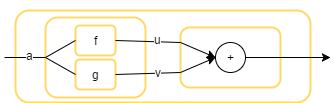
\includegraphics[scale=0.6]{images/addA-comb}
\end{center}
\end{frame}